\chapter{Mod 10 Counter}
\label{chapter:mod10}
\graphicspath{ {./Lab08Mod10Counter/Fig} }

\section{Outcomes and Objectives}

The outcome of this lab is to isimulate a mod10 counter
that will be used as a building block in the implementation
of a digital stopwatch.
Through this process you will achieve the following
learning objectives.
\begin{itemize}
    \item \Paste{bok:CC_Glue_Combo}
    \item \Paste{bok:BMS_RegTran}
    \item \Paste{HDL:Time}
    \item \Paste{HDL:Do}
\end{itemize}

\section{Module: \hdl{mod10Counter}}

A mod 10 counter counts up from 0 to 9 and then rolls over back to 0 to
count up again. The term ``mod'' comes from the word modulus. If you
take a number x and form ``x mod 10'' you get the integer remainder
after division by 10. For example, 12 mod 10 is equal to 2 because 12/10
= 1 with a remainder of 2. Note that ``x mod 10'' will always produce a
value between 0 and 9. Thus, a mod 10 counter will count up from 0 to 9
and then back to 0 to start over again.

You will build the mod 10 counter shown in Figure~\ref{fig:mod10Symbol}. The enb input
enables the counter to count up on a rising edge of the clock. The synch
input causes the mod10Counter to (synchronously) reset of the rising
edge of the clock. The roll output indicated when the currentCount is
going to roll-over from 9 to 0.

\begin{figure}[ht]
    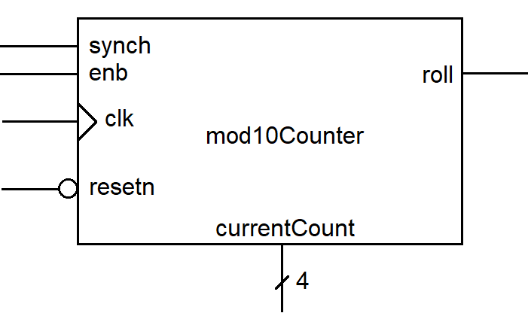
\includegraphics{image1.png}
    \caption{The high-level interface for the mod 10 counter.}
    \label{fig:mod10Symbol}
\end{figure}

Table~\ref{table:mod10StateTable} is the truth table for the currentCount output. When the
\textbf{enb} input is at logic 1, \textbf{currentCount} is incremented
mod 10 on the next positive clk edge. When the \textbf{synch} input
equals 1, \textbf{currentCount} goes to 4'b0000 on the next positive
\textbf{clk} edge. The \textbf{synch} input takes precedence over the
\textbf{enb} input, so if both are at logic 1 then \textbf{currentCount}
goes to 4'b0000 on the next positive \textbf{clk} edge.

\begin{longtable}[]{@{}
        |  >{\raggedright\arraybackslash}p{(\columnwidth - 10\tabcolsep) * \real{0.1358}}|
        >{\raggedright\arraybackslash}p{(\columnwidth - 10\tabcolsep) * \real{0.1358}}|
        >{\raggedright\arraybackslash}p{(\columnwidth - 10\tabcolsep) * \real{0.1358}}|
        >{\raggedright\arraybackslash}p{(\columnwidth - 10\tabcolsep) * \real{0.1358}}|
        >{\raggedright\arraybackslash}p{(\columnwidth - 10\tabcolsep) * \real{0.2530}}|
    >{\raggedright\arraybackslash}p{(\columnwidth - 10\tabcolsep) * \real{0.2037}}|@{}}
    \caption{The truth table for the currentCount output from the
    mod10Counter.}\label{table:mod10StateTable}\tabularnewline
    \toprule()
    \begin{minipage}[b]{\linewidth}\raggedright
        reset
    \end{minipage} &
    \begin{minipage}[b]{\linewidth}\raggedright
        clk
    \end{minipage} &
    \begin{minipage}[b]{\linewidth}\raggedright
        enb
    \end{minipage} &
    \begin{minipage}[b]{\linewidth}\raggedright
        synch
    \end{minipage} &
    \begin{minipage}[b]{\linewidth}\raggedright
        currentCount
    \end{minipage} &
    \begin{minipage}[b]{\linewidth}\raggedright
        Note
    \end{minipage} \\
    \midrule()
    \endfirsthead
    \toprule()
    \begin{minipage}[b]{\linewidth}\raggedright
        reset
    \end{minipage} &
    \begin{minipage}[b]{\linewidth}\raggedright
        clk
    \end{minipage} &
    \begin{minipage}[b]{\linewidth}\raggedright
        enb
    \end{minipage} &
    \begin{minipage}[b]{\linewidth}\raggedright
        synch
    \end{minipage} &
    \begin{minipage}[b]{\linewidth}\raggedright
        currentCount
    \end{minipage} &
    \begin{minipage}[b]{\linewidth}\raggedright
        Note
    \end{minipage} \\
    \midrule()
    \endhead
    0 & x & x & x & 0 & Asynch reset \\ \hline
    1 & 0, 1, ↓ & x & x & currentCount & No clk edge \\ \hline
    1 & ↑ & 0 & 0 & currentCount & Hold \\ \hline
    1 & ↑ & 0 & 1 & 0 & Synch reset \\ \hline
    1 & ↑ & 1 & 0 & (currentCount +1) mod 10 & Count up \\ \hline
    1 & ↑ & 1 & 1 & 0 & Synch reset \\
    \bottomrule()
\end{longtable}

Table~\ref{table:mod10Roll} is the truth table for the roll output. If \textbf{enb} is logic
1 when the \textbf{currentCount} equals 9, the \textbf{roll} output
equals logic 1. In all other cases the \textbf{roll} output should equal
logic 0. Note, the roll output does not depend on the \textbf{clk}, it's
a combinational logic block.

\begin{longtable}[]{@{}
        | >{\raggedright\arraybackslash}p{(\columnwidth - 4\tabcolsep) * \real{0.2307}}|
        >{\raggedright\arraybackslash}p{(\columnwidth - 4\tabcolsep) * \real{0.5385}}|
    >{\raggedright\arraybackslash}p{(\columnwidth - 4\tabcolsep) * \real{0.2307}}|@{}}
    \caption{The truth table for the roll output from the
    mod10Counter.}\label{table:mod10Roll}\tabularnewline
    \toprule()
    \begin{minipage}[b]{\linewidth}\raggedright
        enb
    \end{minipage} &
    \begin{minipage}[b]{\linewidth}\raggedright
        currentCount
    \end{minipage} &
    \begin{minipage}[b]{\linewidth}\raggedright
        roll
    \end{minipage} \\
    \midrule()
    \endfirsthead
    \toprule()
    \begin{minipage}[b]{\linewidth}\raggedright
        enb
    \end{minipage} &
    \begin{minipage}[b]{\linewidth}\raggedright
        currentCount
    \end{minipage} &
    \begin{minipage}[b]{\linewidth}\raggedright
        roll
    \end{minipage} \\
    \midrule()
    \endhead
    1 & currentCount \textless9 & 0 \\ \hline
    1 & currentCount ==9 & 1 \\
    \bottomrule()
\end{longtable}

\section{System Architecture}
Now that you have a solid grasp of how the mod10Counter should work,
let's turn our attention to how this is accomplished. The internal
organization of the mod10Counter is shown in Figure~\ref{fig:mod10sysArch}.
\pagebreak

\begin{figure}[ht]
    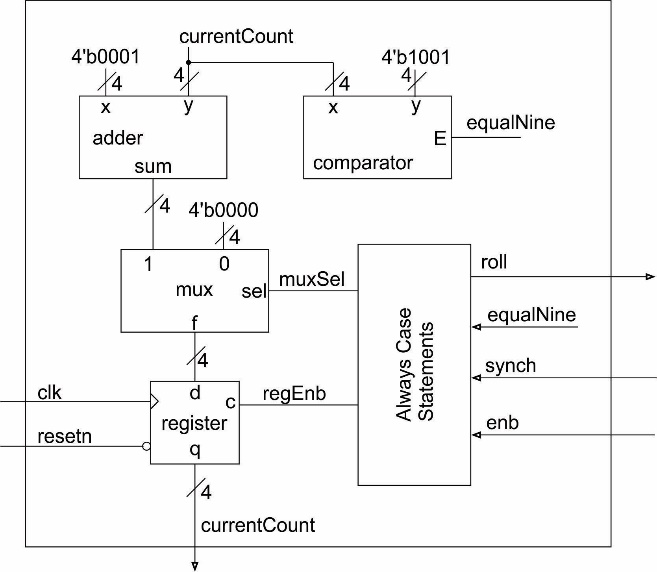
\includegraphics[width=0.6\paperwidth]{image2.jpeg}
    \caption{The internal organization of the mod10counter module.}
    \label{fig:mod10sysArch}
\end{figure}

You have been provided with the adder, comparator, mux, and register
shown in Figure~\ref{fig:mod10sysArch}. In addition to wiring these building blocks together,
you will need to define the logic inside the always/case block.

Use the truth tables in Table~\ref{table:mod10StateTable} and Table~\ref{table:mod10Roll} along with the hardware
organization in Figure~\ref{fig:mod10sysArch} to fill in Table~\ref{table:mod10alwaysCase} .

\begin{longtable}[]{@{}
        | >{\raggedright\arraybackslash}p{(\columnwidth - 10\tabcolsep) * \real{0.1666}}|
        >{\raggedright\arraybackslash}p{(\columnwidth - 10\tabcolsep) * \real{0.1666}}|
        >{\raggedright\arraybackslash}p{(\columnwidth - 10\tabcolsep) * \real{0.1666}}|
        >{\raggedright\arraybackslash}p{(\columnwidth - 10\tabcolsep) * \real{0.1666}}|
        >{\raggedright\arraybackslash}p{(\columnwidth - 10\tabcolsep) * \real{0.1666}}|
    >{\raggedright\arraybackslash}p{(\columnwidth - 10\tabcolsep) * \real{0.1668}}|@{}}
    \caption{The truth table for the always/case logic inside the
    mod10counter.}\label{table:mod10alwaysCase}\tabularnewline\toprule()
    \begin{minipage}[b]{\linewidth}\raggedright
        enb
    \end{minipage} &
    \begin{minipage}[b]{\linewidth}\raggedright
        synch
    \end{minipage} &
    \begin{minipage}[b]{\linewidth}\raggedright
        equalNine
    \end{minipage} &
    \begin{minipage}[b]{\linewidth}\raggedright
        muxSel
    \end{minipage} &
    \begin{minipage}[b]{\linewidth}\raggedright
        regEnb
    \end{minipage} &
    \begin{minipage}[b]{\linewidth}\raggedright
        roll
    \end{minipage} \\
    \midrule()
    \endhead
    0 & 0 & 0 & & & \\ \hline
    0 & 0 & 1 & x & & \\ \hline
    0 & 1 & 0 & & & \\ \hline
    0 & 1 & 1 & & & \\ \hline
    1 & 0 & 0 & & & 0 \\ \hline
    1 & 0 & 1 & & 1 & \\ \hline
    1 & 1 & 0 & & & \\ \hline
    1 & 1 & 1 & & & \\
    \bottomrule()
\end{longtable}

When you code your always/case statement, with a three-bit output and
then have three \hdl{assign} statements that break this 3-bit output
into individual bits for \hdl{muxSel}, \hdl{regEnb} and \hdl{roll}.

\hypertarget{link:mod10Verilog}{}{}
Complete the coding of the \hdl{mod10Counter} instantiating the
the modules in Figure~\ref{fig:mod10sysArch} and including the
always/case statement as a CSA.  Once you complete writing this
code, you will need to demonstrate its proper functioning by
simulating the design.  You will \underline{not} be synthesizing
your design this week, so it's \underline{imperative} that you carefully
examine the output because you will be using this module
in the coming weeks as an element in a larger design.

\section{Testbench}

You will need to demonstrate that your mod10Counter operates correctly
by running the provided testbench. Since we will not be synthesizing
today's module, you must be very focused on ensuring that your
mod10Counter is operating \underline{perfectly} because you will
be using this module as a buidling clock in several coming assignments.
In order for you to verify \underline{perfect} operation, you need to understand
what expected output so that you can compare it to what your simulation actually
producing. Any difference between these two indicate an error (either in
your understanding or circuit behavior) that need to be fixed.

Start by completing the timing diagram in Figure~\ref{fig:mod10TimingDiamgram}
using the value from the testbench.  You will have to open the testbench to
find these values.

\begin{landscape}
    \begin{figure}[ht]
        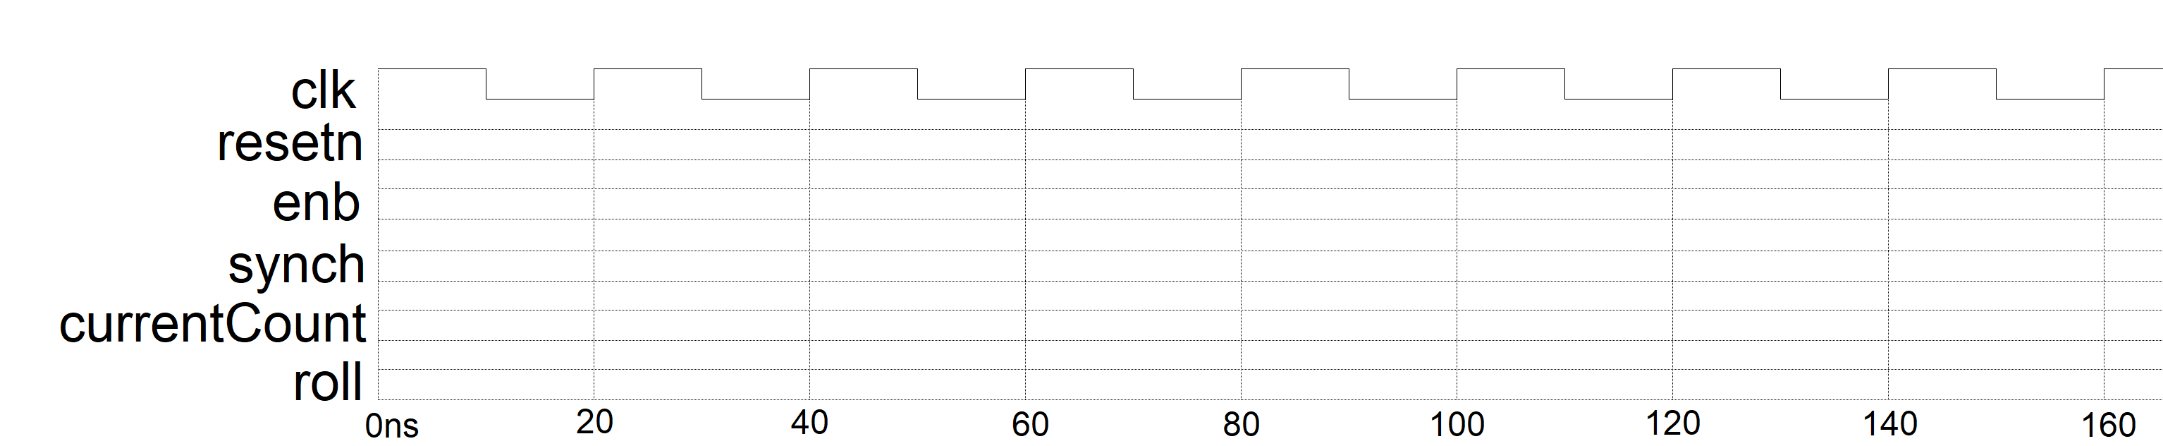
\includegraphics{image4.png}

        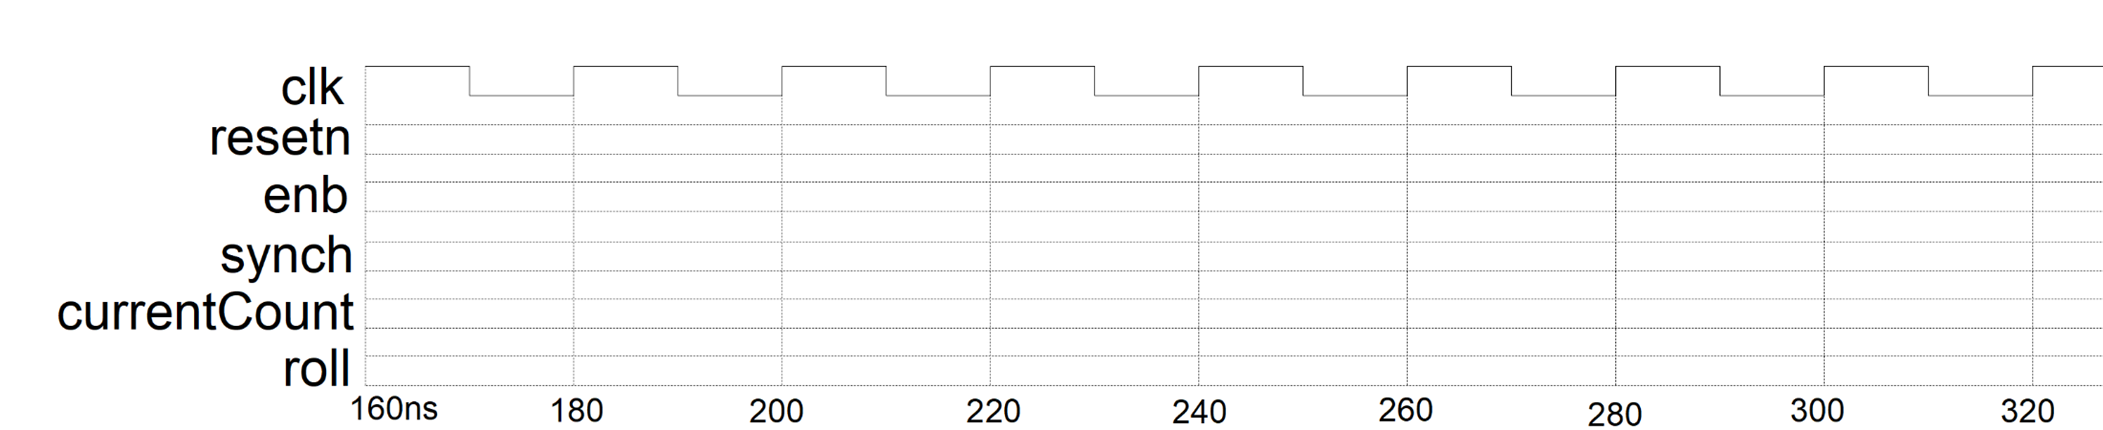
\includegraphics{image5.png}

        \caption{A timing diagram for you to fill out based on the testbench
            code for the mod10Counter. Note the diagram was too wide to be readable
            in one line, so it has been broken at 160ns to make it easier to
        you to read.}
        \label{fig:mod10TimingDiamgram}
    \end{figure}
\end{landscape}

\section{FPGA: Do file}
You have been required to run simulation for almost every lab. This is not
busy-work, all practicing digital designers are expected to demonstrate
proper functionality before modules are incorporated into larger design.
You may have experienced times when you had to run a simulation
multiple times to get your design correct.  You probably got tired setting
up all the signals, colors and radix every time you found an error.  Good
news! You can build a script that does this setup automatically, a do file.
A do file is a script to setup the waveforms for a simulation
including their order, colors and radixes.

Listing 1 shows a partial do file for the mod10counter testbench. The
``\#'' symbol is used to denote comments -- any text placed after them
is ignored by the do file interpreter.

\begin{lstlisting}[language=Verilog,
 caption={A partial do file for the mod10counter.},
basicstyle=\tiny\ttfamily,
 label={listing:mod10Counter},
 frame=single]
############################################
# Search Internet ``modelsim command reference manual''
############################################
vsim work.mod10counter_tb
restart -f
delete wave *

add wave -position end  sim:/mod10counter_tb/uut/clk
        <<you need more add waves here>>
add wave -position end  -radix unsigned -color greenyellow sim:/mod10counter_tb/uut/currentCount
 \end{lstlisting}

The first three lines start the simulation and delete any waveforms that
may be left over from a previous simulation. I included this in the do
file because I sometimes rerun a simulation to observe the modules
behavior at some earlier time.

The waveforms in the simulation are added using the ``add wave''
command. If you drag-and-drop a signal name into the waveform area, you
will see the add wave command appear in the console are at the bottom of
the ModelSim window. For example when I manually added the clk, I see:

\begin{verbatim}
add wave -position end sim:/mod10counter_tb/uut/clk
\end{verbatim}

I then add the color of the wave and the radix in between ``end'' and
``sim''. See Listing 1 for a couple of examples. You should use notepad
to edit the do file. Do NOT use a word processor like MS Word because
they tend to change the extensions of files when you save.

After editing the do file, it should be stored in the following folder:

\begin{verbatim}
<projectDirectory>\mod10Counter\simulation\modelsim
\end{verbatim}

Where \textless projectDirectory\textgreater{} is the path of your
project. If this folder does not exit, then you need to have to run
``Start Analysis and Elaboration'' at least once. You know you are in
the project directory when you see the project QPF file.

When you have the testbench setup in ModelSim, you will
execute the commands in the do file by typing the
following into the console window.  The console is at the
bottom of the ModelSim window.

\begin{verbatim}
do mod10counter_tbWaveSetup.do
\end{verbatim}

The ModelSim console allows tab completion, a feature that helps you
fill-in the characters of long file name. To use tab completion, type
the first few characters of a command/filename and then press Tab. If
there are no other file names that match what you have typed in, the
remainder of the file name will be auto-complete for you. If there is
more than one filename choice, the command/filename will be completed up
to the ambiguity and the console will provide a list of candidate
filenames.

You can issue a variety of commands in the console window.   A very popular
command is ``run \textless time\textgreater'' to simulate some amount
of time.

\section{Testbench}
Edit the do file provided on Canvas to produce the following output.
\hypertarget{link:mod10DoFile}{}{}

\begin{tabular}{p{3cm}p{3cm}p{3cm}}
    signal & radix & signal color \\ \hline
    clk         & default         & green  \\
    reset     & default         & green  \\
    enb         & default         & gold  \\
    synch     & default         & gold  \\
    roll         & default         & yellow  \\
    currentCount     & unsigned & greenyellow  \\
\end{tabular}

You need to look at the values produced by the mod10counter and compare
them against the values in Table~\ref{table:mod10StateTable}. Look for discrepancies
starting at time 0 and only advancing the simulation when everything is
correct. You will have to transcend the design hierarchy to find the
source of your errors. Most errors are due to incorrect wiring or
modules -- wrong names or wrong signal order.

\section{Turn in}

You may work in teams of at most two. Make a record of your response to
the items below and turn them in a single copy as your team's solution
on Canvas using the instructions posted there. Include the names of both
team members at the top of your solutions. Use complete English
sentences to introduce what each of the following listed items (below)
is and how it was derived. In addition to this submission, you will be
expected to demonstrate your circuit at the beginning of your lab
section next week.

\subsubsection{Mod10 Counter Verilog}

\begin{itemize}
    \item
        Complete the truth table in Table~\ref{table:mod10alwaysCase}.
    \item
        Complete hand-drawn timing diagram in Figure~\ref{fig:mod10TimingDiamgram}.
    \item
        \hyperlink{link:mod10Verilog}{Verilog code} for the body of the mode10counter module (courier 8-point
        font single spaced), leave out header comments.
\end{itemize}

\subsubsection{Testbench}
\begin{itemize}
    \item
        Complete \hyperlink{link:mod10Simulation}{simulation timing diagram} of the \hdl{mod10counter}.
    \item
        The contents of your   \hyperlink{link:mod10Simulation}{Do File}.
\end{itemize}
